\begin{figure*}[h]
  \centering

  % Define block styles used later

  \tikzstyle{module}=[draw, draw=blue!80, text width=10em, 
  text centered, minimum height=5em, minimum width = 15em, drop shadow, rounded corners,
  fill=blue!30]
  
  \tikzstyle{vecArrow} = [thick, decoration={markings,mark=at position
    1 with {\arrow[semithick]{open triangle 60}}},
  double distance=1.4pt, shorten >= 5.5pt,
  preaction = {decorate},
  postaction = {draw,line width=1.4pt, white,shorten >= 4.5pt}]

  % Define distances for bordering
  \def\blockdist{1.5}
  \def\edgedist{2.5}

  \begin{tikzpicture}[node distance=3cm,thick,scale=0.4, every node/.style={scale=0.4},path image/.style={
      path picture={
        \node at (path picture bounding box.center) {
          \includegraphics[width=1cm]{#1}
        };}}]
    \tikzstyle{conefill} = [path image=,fill opacity=0.8]
    \node[module=above:pre] (pre) at (4.5,-2.6) {\Large Pre-processing};
    \node[module,below of=pre] (seg) {\Large Segmentation};
    \node[module,below of=seg] (reg) {\Large Registration};

    \path[->,dashed] (seg.west) edge [bend right=70] node {} (reg.west);
    \path[->,dashed] (reg.east) edge [bend right=70] node {} (seg.east);

    \draw[->] (pre)--(seg);
    \draw[->] (seg)--(reg);

    \begin{pgfonlayer}{background}
      \path (pre.west |- pre.north)+(-0.9,1.0+\blockdist) node (a) {};
      \path (reg.east |- reg.south)+(+0.9,-0.5) node (b) {};
      
      \path[fill=blue!10,rounded corners, draw=blue!20, dashed] (a) rectangle (b);
    \end{pgfonlayer}
    
    \path (pre.north) +(0,+\blockdist) node (bgreg) {\Large Image regularization};

    \begin{scope}[node distance=10cm]
      \node[module] (det) [below right=0cm and 3cm of pre] {\Large Features detection};
    \end{scope}
    \begin{scope}[node distance=3.5cm]
      \node[module,above of=det] (roi) {\Large ROIs\\detection/selection};
    \end{scope}
    \node[module,below of=det] (sel) {\Large Features\\selection/extraction};
    \node[module,below of=sel] (cla) {\Large Features\\classification/fusion};

    \draw[->] (roi)--(det);
    \draw[->] (det)--(sel);
    \draw[->] (sel)--(cla);

    \begin{pgfonlayer}{background}
      \path (roi.west |- roi.north)+(-0.25,0.8) node (c) {};
      \path (roi.east |- roi.south)+(+0.25,-0.25) node (d) {};
      
      \path[fill=blue!20,rounded corners, draw=blue!25, dashed] (c) rectangle (d);
    \end{pgfonlayer}

    \path (roi.west |- roi.north) +(.6,0.4) node (bgfea) {\Large \textbf{CADe}};

    \begin{pgfonlayer}{background}
      \path (det.west |- det.north)+(-0.25,0.8) node (c) {};
      \path (cla.east |- cla.south)+(+0.25,-0.25) node (d) {};
      
      \path[fill=blue!20,rounded corners, draw=blue!25, dashed] (c) rectangle (d);
    \end{pgfonlayer}

    \path (roi.west |- det.north) +(.6,0.4) node (bgfea) {\Large \textbf{CADx}};     

    % Define the place where the arrow should start anf finish
    \path (seg.east |- seg.north)+(+0.9,0) node (e) {};
    \path (sel.west |- seg.north)+(-0.8,0) node (f) {};

    \draw[double distance =3pt,preaction={-triangle 90,thin,draw,shorten >=-1mm}] (e) -- (f) node[midway,above] {\Large Regularized data};

    \begin{scope}[yshift=34,xshift=-86]
      \transparent{0.6}\draw[path image=content/proposal/figures/tikzimage/t2.eps] (0,0) rectangle (1.0,1.0);
    \end{scope}

    \begin{scope}[yshift=31,xshift=-83]
      \transparent{0.6}\draw[path image=content/proposal/figures/tikzimage/t2.eps] (0,0) rectangle (1.0,1.0);
    \end{scope}

    \begin{scope}[yshift=28,xshift=-80]
      \transparent{0.8}\draw[path image=content/proposal/figures/tikzimage/t2.eps] (0,0) rectangle (1.0,1.0);
      \path (0,0)+(-1.5,0.3) node {\Large T$_2$-W MRI};
    \end{scope}

    \begin{scope}[yshift=-33,xshift=-86]
      \transparent{0.6}\draw[path image=content/proposal/figures/tikzimage/t2.eps] (0,0) rectangle (1.0,1.0);
    \end{scope}

    \begin{scope}[yshift=-36,xshift=-83]
      \transparent{0.6}\draw[path image=content/proposal/figures/tikzimage/t2.eps] (0,0) rectangle (1.0,1.0);
    \end{scope}

    \begin{scope}[yshift=-39,xshift=-80]
      \transparent{0.8}\draw[path image=content/proposal/figures/tikzimage/t2.eps] (0,0) rectangle (1.0,1.0);
      \path (0,0)+(-1.2,0.3) node {\Large T$_2$ map};
    \end{scope}

    \begin{scope}[yshift=-100,xshift=-86]
      \transparent{0.6}\draw[path image=content/proposal/figures/tikzimage/dce.eps] (0,0) rectangle (1.0,1.0);
    \end{scope}

    \begin{scope}[yshift=-103,xshift=-83]
      \transparent{0.6}\draw[path image=content/proposal/figures/tikzimage/dce.eps] (0,0) rectangle (1.0,1.0);
    \end{scope}

    \begin{scope}[yshift=-106,xshift=-80]
      \transparent{0.8}\draw[path image=content/proposal/figures/tikzimage/dce.eps] (0,0) rectangle (1.0,1.0);
      \path (0,0)+(-1.5,0.3) node {\Large DCE MRI};
    \end{scope}

    \begin{scope}[yshift=-167,xshift=-86]
      \transparent{0.6}\draw[path image=content/proposal/figures/tikzimage/dwi1.eps] (0,0) rectangle (1.0,1.0);
    \end{scope}

    \begin{scope}[yshift=-170,xshift=-83]
      \transparent{0.6}\draw[path image=content/proposal/figures/tikzimage/dwi1.eps] (0,0) rectangle (1.0,1.0);
    \end{scope}

    \begin{scope}[yshift=-173,xshift=-80]
      \transparent{0.8}\draw[path image=content/proposal/figures/tikzimage/dwi1.eps] (0,0) rectangle (1.0,1.0);
      \path (0,0)+(-1.5,0.3) node {\Large DW MRI};
    \end{scope}

    \begin{scope}[yshift=-234,xshift=-86]
      \transparent{0.6}\draw[path image=content/proposal/figures/tikzimage/adc.eps] (0,0) rectangle (1.0,1.0);
    \end{scope}

    \begin{scope}[yshift=-237,xshift=-83]
      \transparent{0.6}\draw[path image=content/proposal/figures/tikzimage/adc.eps] (0,0) rectangle (1.0,1.0);
    \end{scope}

    \begin{scope}[yshift=-240,xshift=-80]
      \transparent{0.8}\draw[path image=content/proposal/figures/tikzimage/adc.eps] (0,0) rectangle (1.0,1.0);
      \path (0,0)+(-1.5,0.3) node {\Large ADC};
    \end{scope}

    \begin{scope}[yshift=-301,xshift=-86]
      \transparent{0.6}\draw[path image=content/proposal/figures/tikzimage/mrsi.eps] (0,0) rectangle (1.0,1.0);
    \end{scope}

    \begin{scope}[yshift=-304,xshift=-83]
      \transparent{0.6}\draw[path image=content/proposal/figures/tikzimage/mrsi.eps] (0,0) rectangle (1.0,1.0);
    \end{scope}

    \begin{scope}[yshift=-307,xshift=-80]
      \transparent{0.8}\draw[path image=content/proposal/figures/tikzimage/mrsi.eps] (0,0) rectangle (1.0,1.0);
      \path (0,0)+(-1,0.3) node {\Large MRSI};
    \end{scope}

    \path (pre.west |- roi.north)+(-3.5,1.0+\blockdist) node (g) {};
    \path (reg.west |- cla.south)+(-3.5,-0.5) node (h) {};

    \draw[decorate,decoration={brace,raise=6pt,amplitude=10pt}, thick]
    (g)--(h) ;
    
    \path (seg.west |- seg.north)+(-2.5,0) node (i) {};
    \path (seg.west |- seg.north)+(-0.9,0) node (j) {};
    
    \draw[double distance =3pt,preaction={-triangle 90,thin,draw,shorten >=-1mm}] (i) -- (j);   

    \path (sel.east |- seg.north)+(2,0) node (k) {};
    \path (sel.east |- seg.north)+(0.5,0) node (l) {};
    
  \end{tikzpicture}
  \caption{Common \ac{cad} framework based on \ac{mri} images used to detect prostate cancer.}
  \label{fig:wkfcad}
\end{figure*}

% \begin{figure*}
%   \centering
%   \hspace*{\fill}
%   \subfigure[\ac{t2w}-\ac{mri} slice of an healthy prostate acquire with a 1.5 Tesla \ac{mri}. The blue contour represents the \ac{cg} while the \ac{pz} corresponds to the green contour.]{\label{subfig:t2whealthy}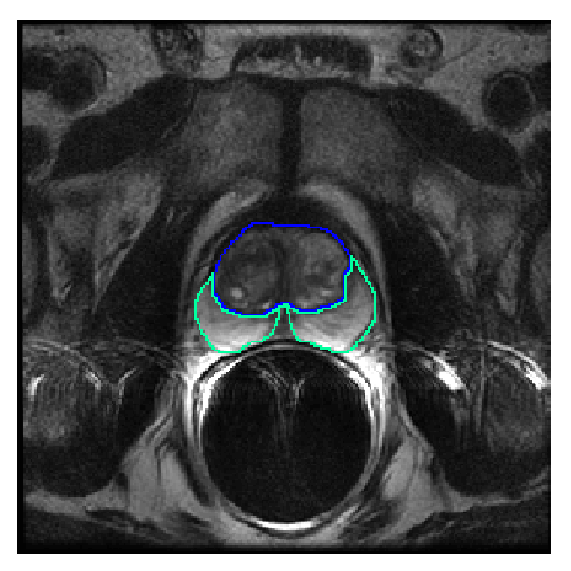
\includegraphics[width=0.3\linewidth]{12_figures/figures/t2w/t2w_healthy.eps}} \hfill
%   \subfigure[\ac{t2w}-\ac{mri} slice of a prostate with a \ac{cap} highlighted in the \ac{pz} using a 3.0 Tesla \ac{mri} scanner.]{\label{subfig:t2wcancerpz}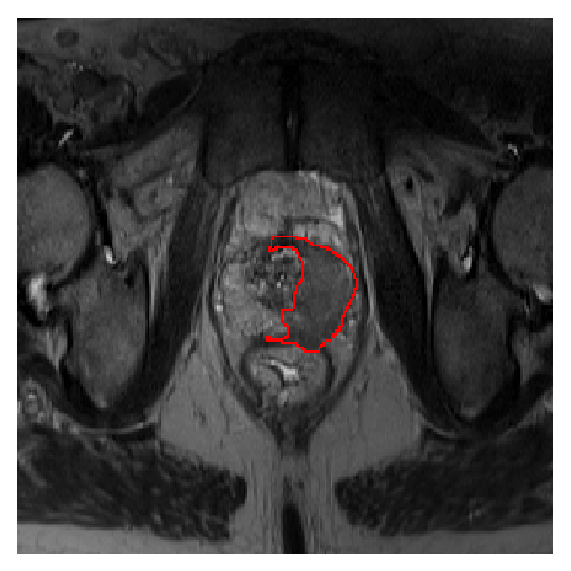
\includegraphics[width=0.3\linewidth]{12_figures/figures/t2w/t2w_cancer_pz.eps}} \hfill
%   \subfigure[\ac{t2w}-\ac{mri} slice of a prostate with a \ac{cap} highlighted in the \ac{cg} using a 3.0 Tesla \ac{mri} scanner.]{\label{subfig:t2wcancercg}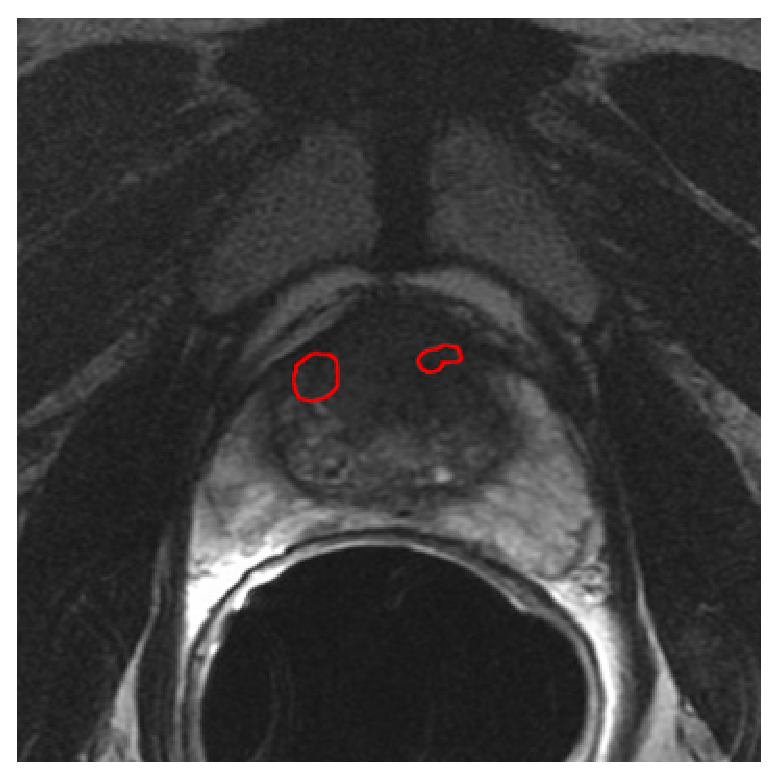
\includegraphics[width=0.3\linewidth]{12_figures/figures/t2w/t2w_cancer_cg.eps}}
%   \hspace*{\fill}
%   \caption{Rendering of \ac{t2w}-\ac{mri} prostate image with both 1.5 and 3.0 Tesla \ac{mri} scanner.}
%   \label{fig:t2w}
% \end{figure*}

% \begin{figure*}
%   \centering
%   \hspace*{\fill}
%   \subfigure[]{\label{subfig:t1w}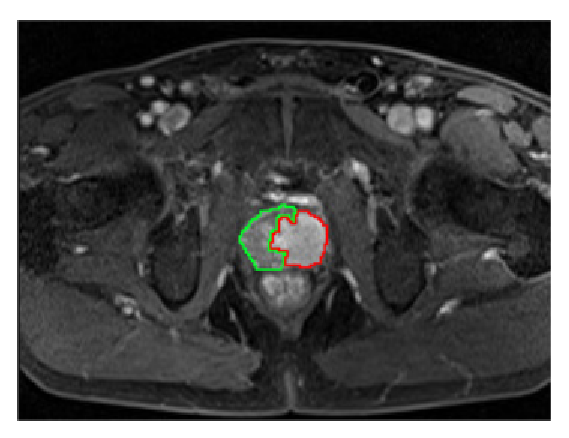
\includegraphics[width=0.35\linewidth]{12_figures/figures/dce/slice.eps}} \hfill
%   \subfigure[]{\label{subfig:dce}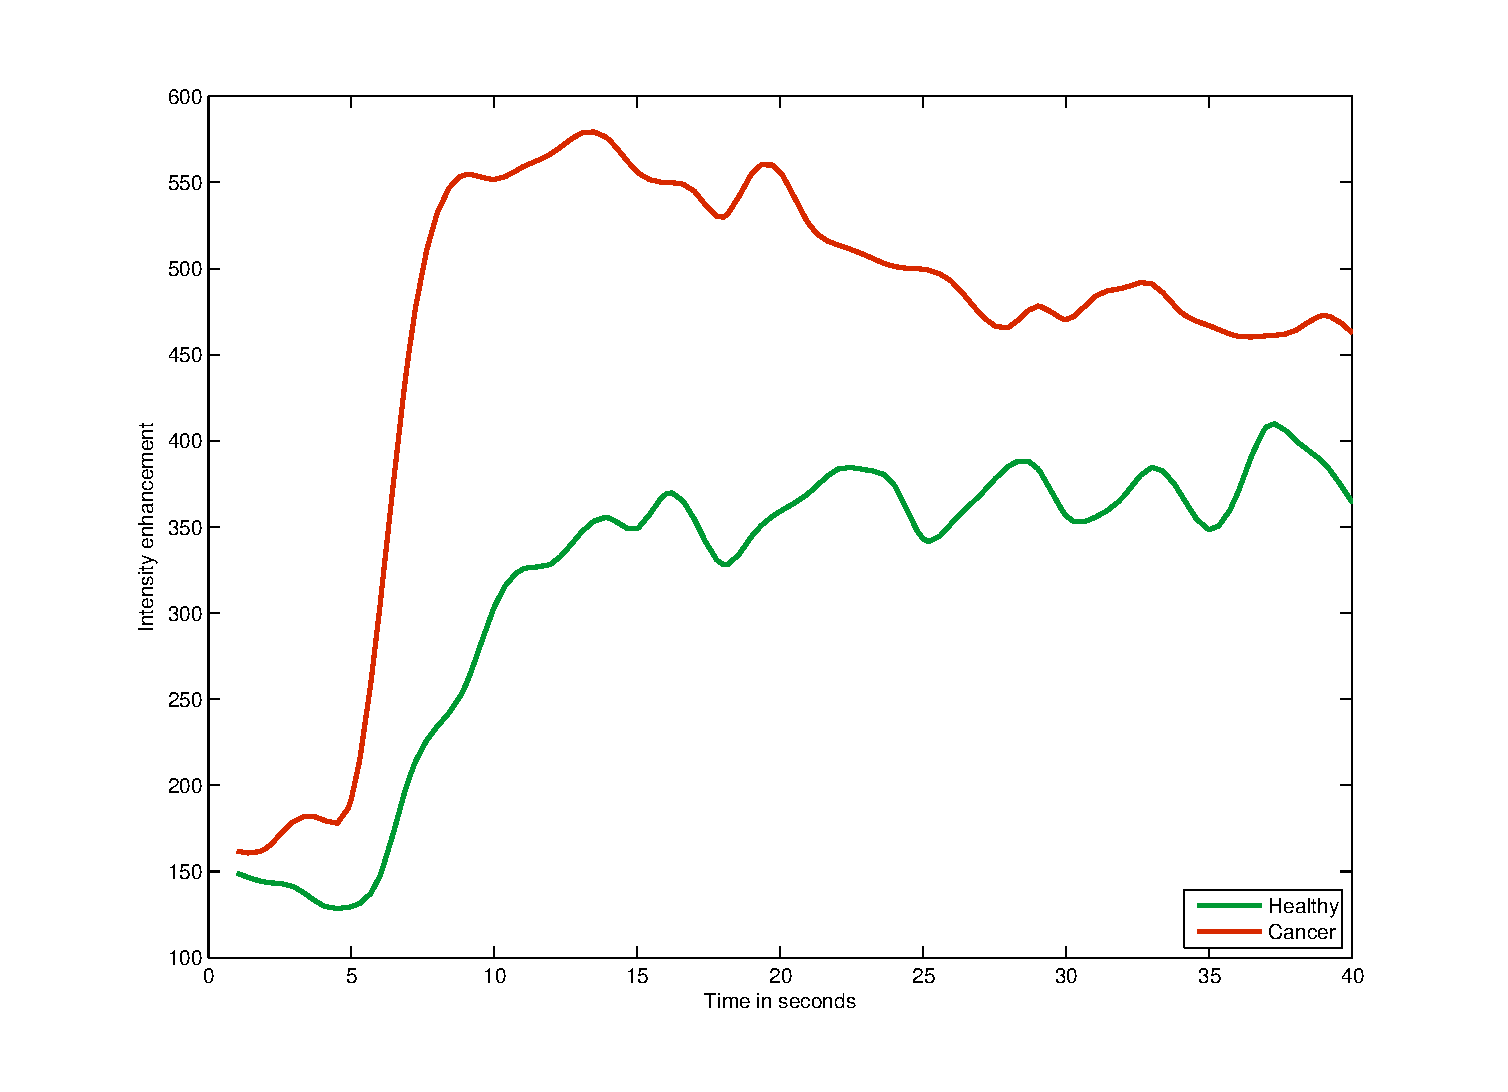
\includegraphics[width=0.35\linewidth]{12_figures/figures/dce/dce_cancer_healthy.eps}}
%   \hspace*{\fill}
%   \caption{Illustration of: \subref{subfig:t1w} \ac{t1w}-\ac{mri} image and \subref{subfig:dce} typical enhancement signals observed in \ac{dce}-\ac{mri} analysis collected with a 3.0 Tesla \ac{mri} scanner. The red curve is typical from \ac{cap} while the green curve is characteristic of healthy tissue.}
%   \label{fig:dceana}
% \end{figure*}

% \begin{figure}
%   \centering
%   \hspace*{\fill}
%   \subfigure[]{\label{subfig:dwi}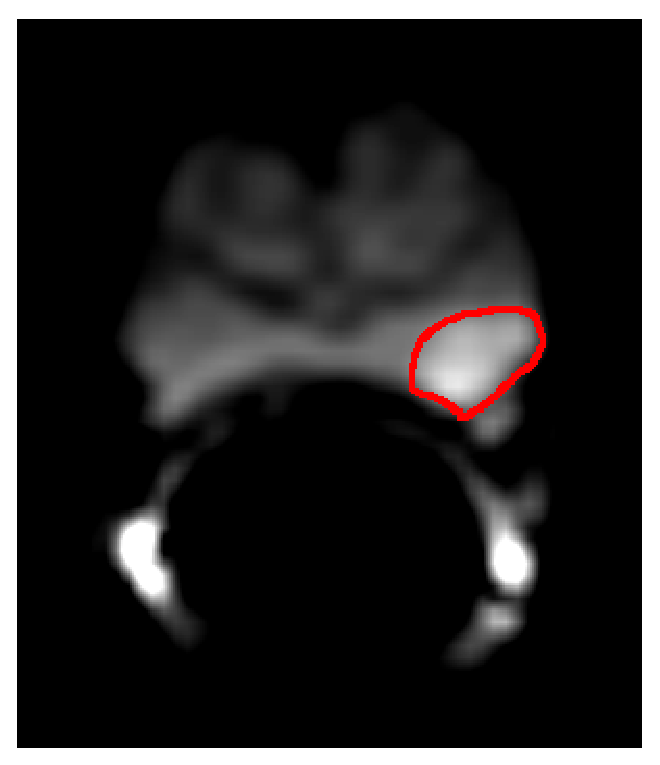
\includegraphics[height=0.15\textheight]{12_figures/figures/dwi/dwi_cancer.eps}} \hfill
%   \subfigure[]{\label{subfig:adc}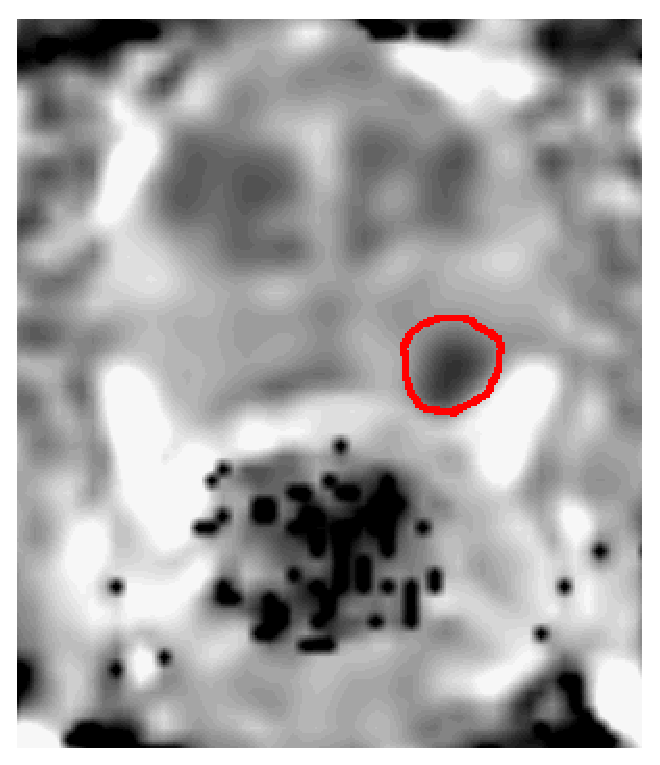
\includegraphics[height=0.15\textheight]{12_figures/figures/dwi/adc_cancer.eps}}
%   \hspace*{\fill}
%   \caption{Illustration of: \subref{subfig:dwi} \ac{dw}-\ac{mri} and \subref{subfig:adc} \ac{adc} map. The signal intensity corresponding to cancer are inversely correlated on these two types of imaging techniques. The cancer is highlighted in red.}
%   \label{fig:dwi}
% \end{figure}

% \begin{figure*}
%   \centering
%   \hspace*{\fill}
%   \subfigure[]{\label{subfig:mrsihea}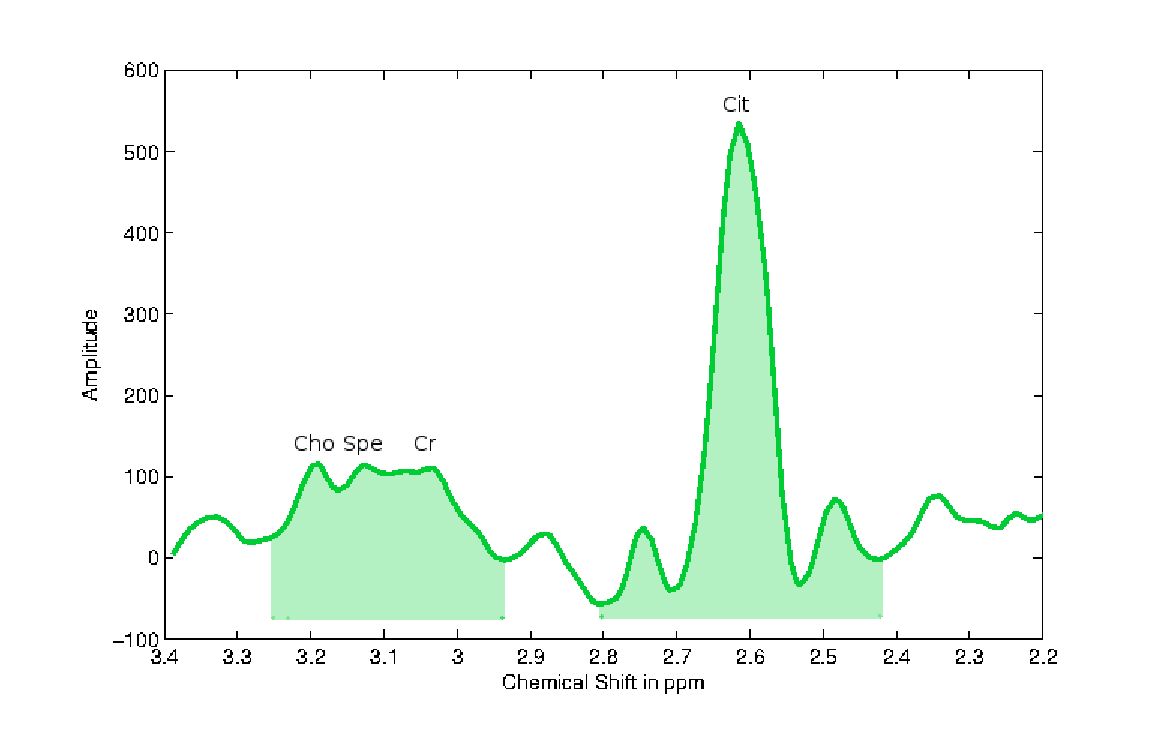
\includegraphics[width=0.45\linewidth]{12_figures/figures/mrsi/mrsi_healthy.eps}} \hfill
%   \subfigure[]{\label{subfig:mrsican}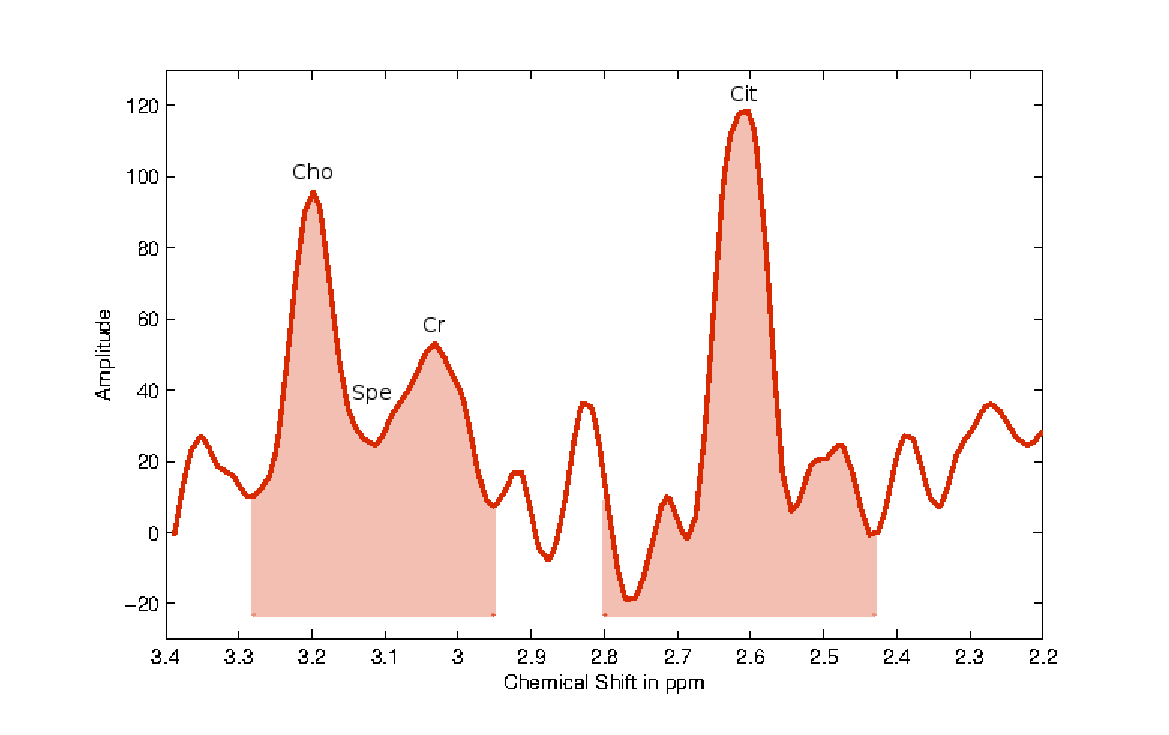
\includegraphics[width=0.45\linewidth]{12_figures/figures/mrsi/mrsi_cancer.eps}}
%   \hspace*{\fill}
%   \caption{Illustration of an \ac{mrsi} spectrum both \subref{subfig:mrsihea} healthy and \subref{subfig:mrsican} cancerous voxel with a 3.0 Tesla \ac{mri}. The highlighted areas corresponds to the related concentration of the metabolites which is computed by integrating the area under each peak. Acronyms: Choline (Cho), Spermine (Spe), Creatine (Cr) and Citrate (Cit).}
%   \label{fig:mrsi}
% \end{figure*}

%%% Local Variables: 
%%% mode: latex
%%% TeX-master: "../../../main"
%%% End: 
